\documentclass[a4paper]{article}
\usepackage[utf8]{inputenc}
\usepackage[spanish, es-tabla, es-noshorthands]{babel}
\usepackage[table,xcdraw]{xcolor}
\usepackage[a4paper, footnotesep = 1cm, width=20cm, top=2.5cm, height=25cm, textwidth=18cm, textheight=25cm]{geometry}
%\geometry{showframe}

\usepackage{tikz}
\usepackage{amsmath}
\usepackage{amsfonts}
\usepackage{amssymb}
\usepackage{float}
\usepackage{graphicx}
\usepackage{caption}
\usepackage{subcaption}
\usepackage{multicol}
\usepackage{multirow}
\setlength{\doublerulesep}{\arrayrulewidth}
\usepackage{booktabs}
\usepackage{mathrsfs,amsmath}
\usepackage{hyperref}
\hypersetup{
    colorlinks=true,
    linkcolor=blue,
    filecolor=magenta,      
    urlcolor=blue,
    citecolor=blue,    
}

\newcommand{\quotes}[1]{``#1''}
\usepackage{array}
\newcolumntype{C}[1]{>{\centering\let\newline\\\arraybackslash\hspace{0pt}}m{#1}}
\usepackage[american]{circuitikz}
\usetikzlibrary{calc}
\usepackage{fancyhdr}
\usepackage{units} 

\graphicspath{./Imagenes}

\pagestyle{fancy}
\fancyhf{}
\lhead{22.05 ASSD}
\rhead{Mechoulam, Lambertucci, Rodriguez, Londero}
\rfoot{Página \thepage}

\begin{document}

%%%%%%%%%%%%%%%%%%%%%%%%%
%		Caratula		%
%%%%%%%%%%%%%%%%%%%%%%%%%

\begin{titlepage}
\newcommand{\HRule}{\rule{\linewidth}{0.5mm}}
\center
\mbox{\textsc{\LARGE \bfseries {Instituto Tecnológico de Buenos Aires}}}\\[1.5cm]
\textsc{\Large 22.05 Análisis de Señales y Sistemas Digitales}\\[0.5cm]


\HRule \\[0.6cm]
{ \Huge \bfseries Trabajo práctico N$^{\circ}$2}\\[0.4cm] 
\HRule \\[1.5cm]


{\large

\emph{Grupo 3}\\
\vspace{3px}

\begin{tabular}{lr} 	
\textsc{Mechoulam}, Alan  &  58438\\
\textsc{Lambertucci}, Guido Enrique  & 58009 \\
\textsc{Rodriguez Turco}, Martín Sebastian  & 56629 \\
\textsc{Londero Bonaparte}, Tomás Guillermo  & 58150 \\
\end{tabular}

\vspace{20px}

\emph{Profesores}\\
Jacoby, Daniel Andres\\
Belaustegui Goitia, Carlos F.\\
Iribarren, Rodrigo Iñaki\\
\vspace{3px}
%\textsc{} \\	

\vspace{100px}

\begin{tabular}{ll}

Presentado: & 15/05/20\\

\end{tabular}

}

\vfill

\end{titlepage}


%%%%%%%%%%%%%%%%%%%%%
%		Indice		%
%%%%%%%%%%%%%%%%%%%%%

%\tableofcontents
%\newpage

%%%%%%%%%%%%%%%%%%%%%
%		Informe		%
%%%%%%%%%%%%%%%%%%%%%

%\begin{center}
%	\Large{\textcolor{red}{\textbf{EN ROJO PONGO LO QUE HAY QUE HACER. NO BORRARLO HASTA NO TERMINARLO. RESPETAR FORMATOS.}} \textcolor{orange}{EN AZUL IDEAS DE QUE DESARROLLAR.}}
%\end{center}

\textbf{\textit{En el siguiente trabajo se presenta el estudio, investigación y análisis de un proceso de seguimiento del movimiento de un objeto en tiempo real, siendo conocida su posición inicial. Se realizaron pruebas tanto con videos como con cámaras web, pudiendo alternar el modo de trabajo.}}

%\textcolor{red}{\textbf{\textit{Resumen: falta mencionar ensayos y resultados.}}}

\section{Introducción}
Una imagen puede ser interpretada como una función bidimensional $f\left( x, y\right)$, donde tanto $x$ como $y$ representan en un plano el espacio visualizado, mientras que la misma función $f\left( x, y\right)$ es la intensidad de la imagen bajo un punto dado. Cuando $x$, $y$ y $f\left( x, y\right)$ son valores cuantizados y discretizados, la imagen se transforma en una imagen digital.

%f(x, y) como un campo vectorial cuya salida es un vector de intensidad y frecuencia
	 	
El procesamiento de dichas se define como el conjunto de técnicas aplicadas a estas imágenes, con el objetivo extraer información de ellas. Estas actividades cubren un campo que abarca un sin fin de aplicaciones, ya que se vale de maquinas capaces de detectar la totalidad del espectro electromagnético. Esto significa que se pueden obtener imágenes generadas por fuentes que captan información la cual para los humanos no se asocian con imágenes propiamente dichas, como lo son las ondas de radio, entre tantas otras.
	
Es posible considerar tres tipos de procesos computarizados en el procesamiento de imágenes, basándose en el nivel de tratamiento que se aplique, siendo así clasificados en bajo, medio y alto nivel. Los primeros incluyen actividades tales como reducción de ruido y aumento de contraste, tareas caracterizadas por el hecho de que tanto la entrada como la salida son imágenes. Las actividades de medio nivel de procesamiento incluyen trabajos de segmentación, es decir, identificar regiones u objetos dentro de las imágenes, descripción y clasificación de dichos elementos. Es así que esta categoría es destacada por sus salidas, ya que suelen ser información extraída de las imágenes a la entrada. Por último, los procesos de alto nivel se caracterizan por no solo reconocer objetos y analizarlos, sino también por darles un tratado normalmente asociado con la visión, tales así como ``darles sentido'' \cite{ref:intro1}.
	
%\textcolor{red}{Debe haber suficiente material para que un profesional que no conoce el tema para nada, pueda entenderlo. Referenciar libros y tutorial papers que profundicen.}
	
\section{Investigación}
Dada una señal continua a la entrada del sistema, una imagen sufre de dos procesos claves: \textbf{cuantización} y \textbf{discretización}. Si bien ambos refieren a tomar variables continuas y almacenarlas en memoria como variables discretas, se realiza esta diferenciación entre ambas ya que la primera hace referencia a la amplitud de la señal mientras que la segunda a coordenadas, que para el caso del estudio de imágenes, se refiere a pixeles, siendo estos el mínimo elemento que compone una imagen digital.
	
Ejemplificando lo anterior, se toma una entrada al sistema, como puede ser la presentada en la Figura (\ref{fig:disc1}), la cual, como ya se ha mencionado, es continua en $x$, $y$ y $f(x,y)$.
\begin{figure}[H]
\centering
	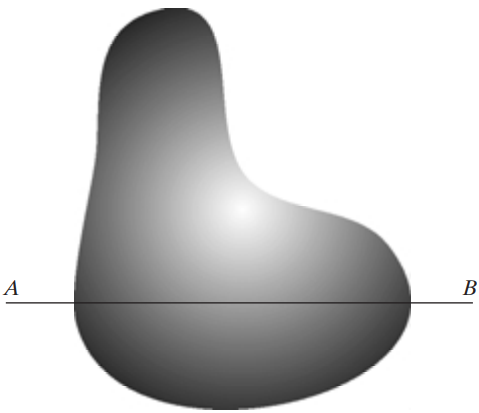
\includegraphics[width=0.3\textwidth]{Imagenes/Digitalizacion_1.png}
	\caption{Entrada continua al sistema.}
	\label{fig:disc1}
\end{figure}

Por lo tanto, se deben tomar coordenadas finitas, por ejemplo, aquellas que se encuentran sobre la recta AB, y asignarle a cada una un valor dado de amplitud. En la Figura~(\ref{fig:disc2}) se observa como una recta continua paralela al eje $x$ (horizontal), la cual posee ciertas variaciones aleatorias dadas por el ruido existente, es dividida en una cierta cantidad de posiciones equiespaciadas (discretización), marcadas con cuadrados blancos sobre la curva, asignándoles un nivel específico en la escala de grises (cuantización), marcado con una linea negra por la izquierda de dicha escala.
\begin{figure}[H]
\centering
	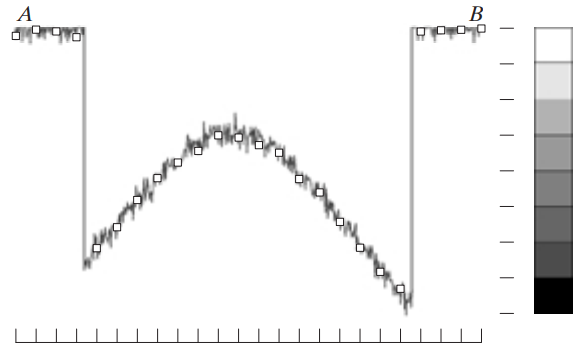
\includegraphics[width=0.4\textwidth]{Imagenes/Digitalizacion_2.png}
	\caption{Amplitud de la escala de grises en la recta AB y muestreo de valores.}
	\label{fig:disc2}
\end{figure}

Realizando el mismo proceso para todos los niveles de discretización en el eje $y$ (vertical), se obtiene finalmente una imagen digitalizada, la cual se la compara a continuación con la original \cite{ref:digit1}.
\begin{figure}[H]
\centering
	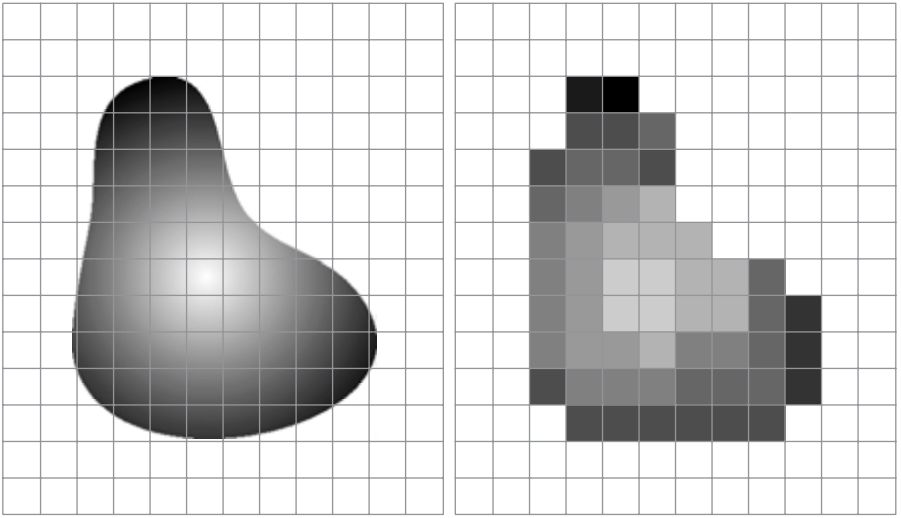
\includegraphics[width=0.5\textwidth]{Imagenes/Digitalizacion_3.png}
	\caption{Imagen original comparada con la imagen digitalizada a procesar.}
	\label{fig:disc3}
\end{figure}

\textcolor{red}{
\begin{itemize}
	%\item Descripción de las líneas de investigación (con referencias).
	\item Descripción de los conceptos más importantes de cada una.
	\item Análisis propio de lo presentado.
	\item Simulaciones de lo más relevante (códigos como apéndice).
	\item Elección del camino y justificación.
\end{itemize}
}
\textcolor{red}{Ehh... es necesario estos 4 puntos que quedaron? Yo pondría solo el código o algo así.}

Este trabajo se centra en procesos de medio nivel. Dicha definición es muy amplia, por lo cual es necesario acotar este camino. Es por ello que se decidió centralizarse en el seguimiento de objetos en imágenes en movimiento. Se busco que, dada ciertas condiciones iniciales conocidas (brindadas por el usuario) en una imagen en movimiento en tiempo real, tomar un conjunto de datos de $x$, $y$ y $f(x,y)$ para así seleccionar un elemento y seguir su movimiento a través del tiempo. 

Se emplearon distintos algoritmos que en conjunto permiten lograr el seguimiento deseado. Se decidió volcarse por el uso de una técnica de detección de flujo óptico\footnote{Patrón de movimiento aparente entre objetos en una escena. Esta técnica extrae la información tanto de elementos estáticos como en movimiento\cite{ref:optic-flow}.}. % de Lucas-Kanade.
Primero se distinguen puntos pertenecientes a un objeto a través del algoritmo de detección de bordes de Shi-Tomasi para luego emplear el método piramidal de Lukas-Kanade. Este consta del uso de información obtenida a partir de la intensidad del gradiente espacial para buscar la posición que mejor se acomoda a una imagen en movimiento \cite{ref:lucas-kanade} \cite{ref:lucas-kanade2}.

Por su lado, se valió del uso de filtros de Kalman. Esta técnica consiste en un algoritmo que elabora una estimación de unas variables deseadas, mediante el uso de una serie de observaciones a lo largo del tiempo. Este filtro considera ciertas imprecisiones en las mediciones, como lo puede ser el ruido existente. La idea del uso de este algoritmo se basa en el hecho de poder estimar la posición de un objeto una vez perdido de vista.
\textcolor{orange}{Escribí una brevísima descripción de lo que se va a hacer. Profundizar y escribir el objetivo final. Justificar elección. \textbf{Yo creo que se puede hablar más de Lucas-Kanade y de Kalman}.}

\section{Aportes}
Se decidió implementar código en \textbf{Python}, apoyándose en la librería \href{https://opencv.org/}{OpenCV}.

Primero se desarrolló un programa capaz de realizar la estimación de una variable mediante el uso del filtro de Kalman. Se puede observar el funcionamiento del algoritmo a continuación: se comparan dos curvas, por un lado una senoidal con un ruido gaussiano montado sobre ella, simulando una medición imprecisa, y por el otro lado, la estimación obtenida a partir del filtro desarrollado.
\begin{figure}[H]
\centering
	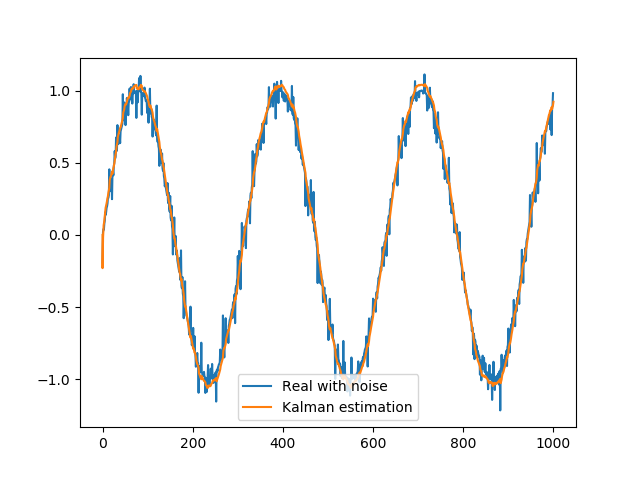
\includegraphics[width=0.4\textwidth]{Imagenes/Kalman_test_1.png}
	\caption{Coseno con ruido comparada con estimación de Kalman.}
	\label{fig:kalman-comp}
\end{figure}

Por otro lado, se obtuvo un algoritmo basado en los elementos mencionados previamente que permite detectar un objeto a partir de su color. El programa logrado permite al usuario seleccionar un área rectangular obtenida de una cámara o un video, siendo los elementos dentro de dicha sección los cuales son seguidos. De esta forma se pueden generar dos ventanas: donde simplemente se muestra el seguimiento del objeto en cuestión y otra resultante de lo denominado ``modo de debug'', en la cual se observa el proceso de optical flow.
\begin{figure}[H]
\centering
	\begin{subfigure}{.4\textwidth}
		\centering
		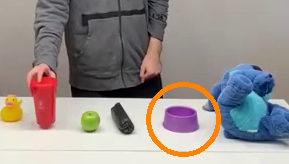
\includegraphics[width=\textwidth]{Imagenes/Optical1.png}
		\caption{Modo normal.}
		\label{fig:optical1}
	\end{subfigure}
	\begin{subfigure}{.4\textwidth}
		\centering
		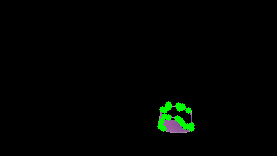
\includegraphics[width=\textwidth]{Imagenes/Optical2.png}
		\caption{Modo debug.}
		\label{fig:optical2}
	\end{subfigure}
	\caption{Resultado de la selección de un elemento.}
	\label{fig:optical12}
\end{figure}

De este modo, se observa en la Figura (\ref{fig:optical1}) como se denota un objeto a seguir, mientras que la Figura (\ref{fig:optical2}) muestra dos datos importantes. Por un lado, se observa en el mismo color del objeto seleccionado como se lo visualiza mediante optical flow, mientras que por otro lado, se muestran los puntos elegidos por el algoritomo de Shi-Tomasi en forma de puntos verdes, los cuales sirven para calcular el centro de masa a seguir. Cabe destacar que el filtro de Kalman estima la posición de este último.
%Luego se buscó utilizar el código previamente mencionado para estimar el movimiento de un objeto en tiempo real. Es así que se realizó un software que 

El programa desarrollado permite elegir al usuario si desea o no ver la ventana en modo debug, la cual además informa sobre la posición del centro de masa. Para elegir un objeto es tan sencillo como seleccionar una área por sobre este, la cual aparece denotada en azul, para luego iniciar el seguimiento presionando al tecla ``espacio''. Por otra parte, el programa permite reelegir un elemento a detectar presionando la tecla ``r''.

%NO SÉ SI ESTÁ BIEN MENCIONAR EL CÓMO USAR EL PROGRAMA ACÁ

\textcolor{red}{
\begin{itemize}
	\item Descripción y análisis de lo original producido por el grupo.
	\item Simulaciones que justifiquen las ideas, y que prueben su originalidad.
	\item Análisis de resultados
\end{itemize}
}

\section{Desarrollo}
\textcolor{red}{
\begin{itemize}
	\item Viabilidad, caminos alternativos.
	\item Proceso de implementación
	\item Documentación de los resultados: Resumen de lo más relevante, demos y programas van al apéndice.
	\item Evaluación y conclusiones del desarrollo.
\end{itemize}
}


\begin{thebibliography}{9}

\bibitem{ref:intro1}
R. C. Gonzalez, R. E. Woods y S. L. Eddins. \textit{Digital Image Processing Using MATLAB}. Prentice Hall, 2da ed, 2002.%, pp. 2-3.

\bibitem{ref:digit1}
R. C. Gonzalez, R. E. Woods y S. L. Eddins. \textit{Digital Image Processing Using MATLAB}. Prentice Hall, 2da ed, 2002, pp. 52-54.

\bibitem{ref:optic-flow}
D. H. Warren y Edward R. Strelow. \textit{Electronic Spatial Sensing for the Blind: Contributions from Perception}. Springer Netherlands, 1er ed, 1985. pp. 414.

\bibitem{ref:lucas-kanade}
B. D. Lucas y T. Kanade. \textit{An iterative image registration technique with an application to stereo vision}. De Proceedings of Imaging Understanding Workshop, pp. 121-130.

\bibitem{ref:lucas-kanade2}
W.S.P. Fernando, L. Udawatta , P. Pathirana. \textit{Identification of Moving Obstacles with Pyramidal
Lucas Kanade Optical Flow and k means
Clustering}. Faculty of Engineering, University of Moratuwa, Sri Lanka.

\end{thebibliography}

\end{document}